\section{Experimental Findings}
\label{sec:findings}


\begin{table*}[!ht]
  \centering

  \begin{tabular}{c c c c c}
    \hline
    Model & ROUGE-1 & ROUGE-2 & ROUGE-L & BERTScore \\
    \hline
    BART w/ Unlimiformer (1,024) & 53.4 & 22.5 & 22.5 & 66.0 \\
    PRIMERA w/ Unlimiformer (4,096) & 56.5 & 24.8 & 26.3 & 67.7 \\
    Hepos (10,240) & 51.34 & 19.09 & \textbf{48.73} & - \\
    PEGASUS-X w/ Staggered & 60.3 & \textbf{30.0} & 31.5 & - \\
    Block-Local Attention (16k) & & & & \\
    LLaMA-7B w/ Positional & 60.0 & 28.0 & 29.5 & - \\
    Interpolation (15k) & & & & \\
    \hline
    Summarization w/ Extraction & \textbf{61.99} & 18.52 & 38.46 & \textbf{86.20} \\
    + GPT-3.5 Turbo (4,096) & & & & \\
    Central truncation + LongT5 (4,096) & 46.20 & 4.38 & 38.27 & \textbf{82.19} \\
    Skimming w/ post-sampling & 46.76 & 4.56 & 39.61 & \textbf{81.96} \\
    removal + LongT5 (4,096) & & & & \\
    \hline
  \end{tabular}

  \caption{
    Automatic evaluation results on the GovReport dataset. Context size of the models are mentioned in parentheses.
    The best score in each metric category is highlighted in \textbf{bold}.
    Results of our algorithms are below the horizontal line in the middle.
  }
  \label{tab:govreport}
\end{table*}

\begin{table*}[!ht]
  \centering

  \begin{tabular}{c c c c c}
    \hline
    Model & ROUGE-1 & ROUGE-2 & ROUGE-L & BERTScore \\
    \hline
    BigBird-Pegasus (16k) & \textbf{60.64} & \textbf{42.46} & \textbf{50.01} & - \\
    \hline
    Skimming w/ pre-sampling & 27.40 & 3.31 & 21.25 & \textbf{82.62} \\
    removal + GPT-3.5 Turbo (4,096) & & & & \\
    Central truncation + GPT-3.5 Turbo (4,096) & 27.77 & 3.09 & 20.56 & \textbf{82.57} \\
    Skimming w/ post-sampling & 26.16 & 2.13 & 20.21 & \textbf{82.40} \\
    removal + GPT-3.5 Turbo (4,096) & & & & \\
    \hline
  \end{tabular}

  \caption{
    Automatic evaluation results on the BigPatent dataset. Context size of the models are mentioned in parentheses.
    The best score in each metric category is highlighted in \textbf{bold}.
    Results of our algorithms are below the horizontal line in the middle.
  }
  \label{tab:bigpatent}
\end{table*}

We test our pipelines with the following models: \textbf{BART} (Bidirectional and Autoregressive Transformer) \cite{lewis-etal-2020-bart} fine-tuned on the CNN/Daily Mail dataset \cite{nallapati2016abstractive} with a context size of 1024, \textbf{LongT5} \cite{guo2021longt5}, a variant of T5 (Text-to-Text Transfer Transformer) \cite{raffel2020exploring}, fine-tuned on the BookSum dataset with a context size of 4096, and \textbf{GPT-3.5 Turbo} \cite{brown2020language} with a context size of 4096.

We compare our results with the state-of-the-art summarization models on the GovReport dataset, including Unlimiformer \cite{bertsch2023unlimiformer} integrated with BART \cite{lewis-etal-2020-bart} and PRIMERA \cite{beltagy2020longformer}, Hepos \cite{huang-etal-2021-efficient}, PEGASUS-X with staggered block-local attention \cite{phang2022investigating}, extended	LLaMA-7B with positional interpolation \cite{chen2023extending}.
We also compare our results with BigBird-Pegasus \cite{zaheer2020big} on the BigPatent dataset.
Refer to \autoref{tab:govreport} and \autoref{tab:bigpatent} for results on the GovReport and BigPatent datasets, respectively.

We were unable to obtain the BERTScores of our baselines, except for Unlimiformer, due to unavailability of code or computational limitations.


\subsection*{Time complexity analysis}

We evaluate the time complexity of our methods by measuring the mean time taken to process a document (excluding the time taken by the model to generate the summaries).
We find that "Central Truncation" (\autoref{method:truncation}) and "Document Skimming" (\autoref{method:skimming}) take approximately the same time.
"Skimming with post-sampling removal" (removing segments after sampling) takes slightly more time than the other two methods.
We can see a significant increase in time taken by "Skimming with pre-sampling removal" (removing segments after sampling) and "Summarization with Keyword Extraction" (\autoref{method:keyword}) due to the additional computations required.
\autoref{fig:times} illustrates the average time taken by our methods.
Check \autoref{tab:encoder-times} for exact values rounded off to two decimal places.

\begin{figure}[!ht]
  \centering
  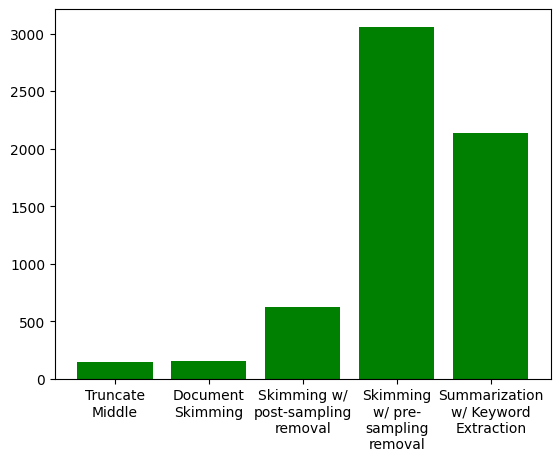
\includegraphics[width=.48\textwidth]{images/encoder-times.png}
  \caption{Mean time taken (in milliseconds) per document using BART tokenizer on BigPatent dataset}
  \label{fig:times}
\end{figure}

\begin{table}[!ht]
  \centering

  \begin{tabular}{c c}
    \hline
    Method & Mean time taken \\
    \hline
    Central Truncation & 142.50 ms \\
    Document Skimming & 155.42 ms \\
    Skimming w/ post- & 625.17 ms \\
    sampling removal & \\
    Skimming w/ pre- & 3059.63 ms \\
    sampling removal & \\
    Summarization & 2131.40 ms \\
    w/ Extraction & \\
    \hline
  \end{tabular}

  \caption{Mean time taken (in milliseconds) per document using BART tokenizer on BigPatent dataset}
  \label{tab:encoder-times}
\end{table}
